\documentclass[tikz,border=10pt]{standalone}
\usepackage{tikz}
\usetikzlibrary{shapes, arrows.meta, positioning, fit, calc, backgrounds, shadows, decorations.markings}

% --- 配色方案 ---
\definecolor{cWorkFill}{RGB}{255, 250, 245} \definecolor{cWorkDraw}{RGB}{230, 81, 0}
\definecolor{cStageFill}{RGB}{245, 250, 255} \definecolor{cStageDraw}{RGB}{1, 87, 155}
\definecolor{cLocalFill}{RGB}{245, 255, 245} \definecolor{cLocalDraw}{RGB}{27, 94, 32}
\definecolor{cRemoteFill}{RGB}{250, 245, 250} \definecolor{cRemoteDraw}{RGB}{74, 20, 140}
\definecolor{lineColor}{RGB}{60, 60, 60}

\tikzset{
    font=\footnotesize\sffamily,
    % --- 容器 ---
    container/.style={
        rectangle, thick, rounded corners=4pt,
        align=center,
        drop shadow={opacity=0.08},
        minimum width=3.0cm,
        minimum height=2.6cm, 
        inner sep=5pt,
    },
    styleWork/.style={ container, draw=cWorkDraw, fill=cWorkFill },
    styleStage/.style={ container, draw=cStageDraw, fill=cStageFill },
    styleLocal/.style={ container, draw=cLocalDraw, fill=cLocalFill },
    styleRemote/.style={ container, draw=cRemoteDraw, fill=cRemoteFill, dashed },
    %
    % --- 内部元素 ---
    card/.style={
        rectangle, draw=black!20, fill=white,
        rounded corners=2pt, inner sep=2pt,
        minimum width=2.0cm, minimum height=0.45cm,
        font=\scriptsize\ttfamily, align=left,
        drop shadow={opacity=0.05}
    },
    statusLabel/.style={
        font=\scriptsize\bfseries\itshape, 
        text=gray!80, anchor=north, yshift=-3pt
    },
    %
    % --- 连线与标签 ---
    conn/.style={
        draw=lineColor, line width=0.8pt,
        -{Latex[length=2mm, width=1.2mm]},
        font=\scriptsize\sffamily
    },
    connDashed/.style={
        conn, dashed, draw=gray!80
    },
    cmdLabel/.style={
        midway, fill=white, text=lineColor, 
        inner sep=1.5pt, rounded corners=2pt,
        align=center, font=\scriptsize\ttfamily,
        opacity=0.8, text opacity=1
    }
}

\begin{document}
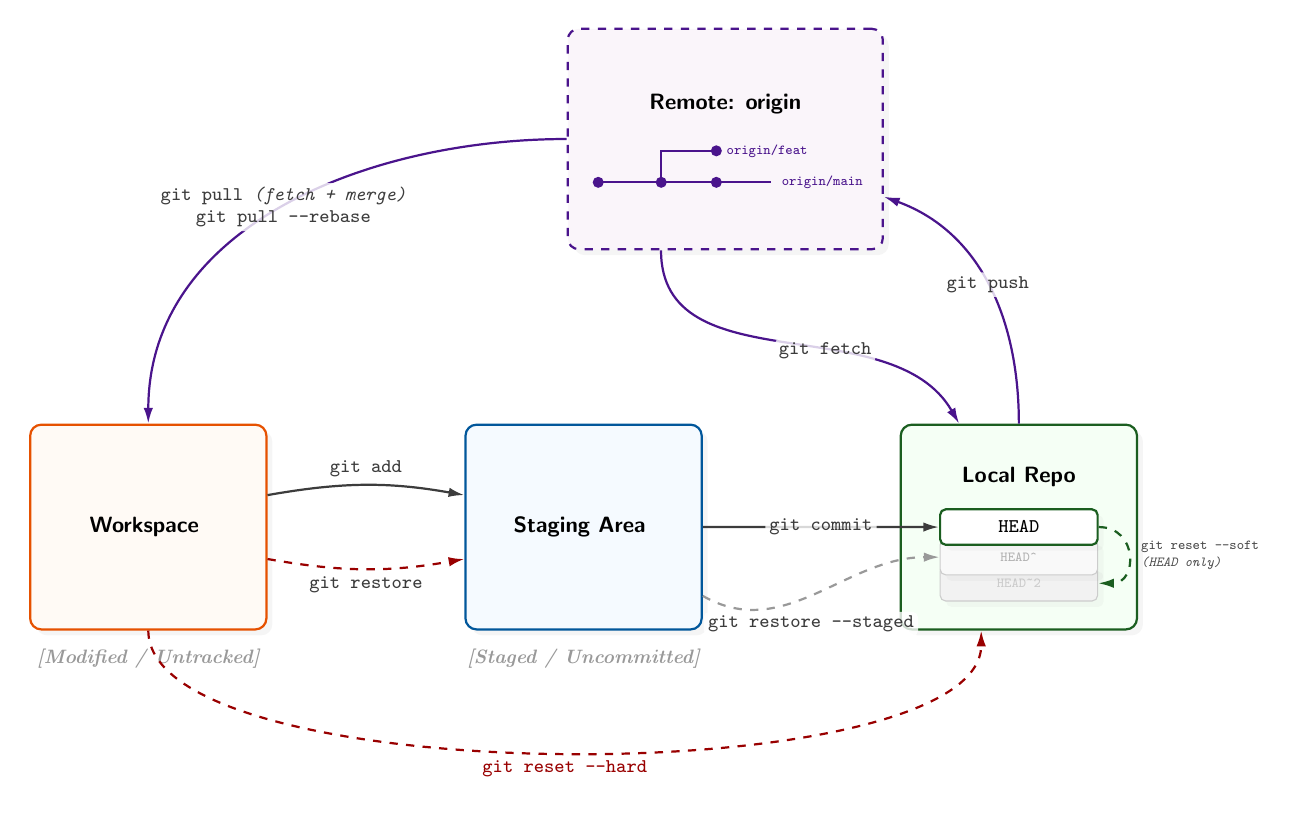
\begin{tikzpicture}[node distance=1.2cm and 2.5cm]

	% =========================================
	% 1. 区域定义
	% =========================================

	% Workspace
	\node [styleWork] (work) {
		\textbf{Workspace}
	};
	\node [statusLabel] at (work.south) {[Modified / Untracked]};

	% Staging
	\node [styleStage, right=of work] (stage) {
		\textbf{Staging Area}
	};
	\node [statusLabel] at (stage.south) {[Staged / Uncommitted]};

	% Local Repo
	\node [styleLocal, right=of stage] (local) {
		\textbf{Local Repo}\\
		\vspace{1.0cm}
	};

	% Remote Repo
	\node [styleRemote, above=2.2cm of stage, xshift=1.8cm, minimum width=4.0cm, minimum height=2.8cm] (remote) {
		\textbf{Remote: origin} \\
		\vspace{0.6cm}
	};

	% =========================================
	% 2. 内部结构可视化
	% =========================================

	% --- Local Commit Stack ---
	\node[card, fill=gray!10, text=gray!40] at ($(local.south) + (0, 0.6)$) (c2) {\tiny HEAD\textasciitilde 2};

	\node[card, fill=gray!5, text=gray!60] at ($(c2.north) + (0, 0.1)$) (c1) {\tiny HEAD\textasciicircum};

	% HEAD
	\node[card, draw=cLocalDraw, thick] at ($(c1.north) + (0, 0.15)$) (c0) {\scriptsize \textbf{HEAD}};

	% --- Remote Branch Tree ---
	\begin{scope}[shift={($(remote.west) + (0.4, -0.55)$)}]
		\draw[cRemoteDraw, thick] (0,0) -- (2.2,0) node[right, font=\tiny\ttfamily] {origin/main};
		\draw[cRemoteDraw, thick] (0.8,0) -- (0.8,0.4) -- (1.5,0.4) node[right, font=\tiny\ttfamily] {origin/feat};
		\fill[cRemoteDraw] (0,0) circle(2pt);
		\fill[cRemoteDraw] (0.8,0) circle(2pt);
		\fill[cRemoteDraw] (1.5,0) circle(2pt);
		\fill[cRemoteDraw] (1.5,0.4) circle(2pt);
	\end{scope}

	% =========================================
	% 3. 核心连线
	% =========================================

	% [Add]
	\draw [conn] (work.15) to[out=10, in=170] node[cmdLabel, above=1pt] {git add} (stage.165);

	% [Commit]
	\draw [conn] (stage.east) to[out=0, in=180] node[cmdLabel, fill=white, opacity=0.8] {git commit} (c0.west);

	% [Push]
	\draw [conn, thick, color=cRemoteDraw] (local.north) to[out=90, in=340] node[cmdLabel, pos=0.5] {git push} (remote.340);

	% =========================================
	% 4. 撤销/回退连线
	% =========================================

	% [Restore Work]
	\draw [connDashed, red!60!black] (work.345) to[out=350, in=190] node[cmdLabel, below=1pt] {git restore} (stage.195);

	% [Restore Staged]
	\draw [connDashed] (stage.330) to[out=330, in=180] node[cmdLabel, fill=white, opacity=0.8, below=6pt, xshift=-2pt, align=left] {git restore -{}-staged} (c1.west);

	% [Reset Soft]: Local Internal Jump (HEAD -> HEAD~2)
	\draw [connDashed, cLocalDraw] (c0.east) to[out=0, in=0, looseness=1.8]
	node [right, pos=0.5, font=\tiny\ttfamily, color=black!70, align=left, xshift=1pt] {
	git reset -{}-soft\\
	\itshape (HEAD only)
	} (c2.east);

	% [Reset Hard]: Work -> Local
	\draw [connDashed, red!60!black] (work.270) to[out=270, in=270, looseness=0.5]
	node[cmdLabel, below=1pt, text=red!60!black] {git reset -{}-hard}
	(local.250);

	% =========================================
	% 5. 远程连线
	% =========================================

	% [Pull]
	\draw [conn, thick, color=cRemoteDraw] (remote.180) to[out=180, in=90]
	node[cmdLabel, pos=0.5] {
		git pull \itshape (fetch + merge) \\
		git pull --rebase
	} (work.north);

	% [Fetch]
	\draw [conn, thick, color=cRemoteDraw] (remote.240) to[out=270, in=120] node[cmdLabel, pos=0.6, fill=white] {git fetch} (local.120);

\end{tikzpicture}
\end{document}